\documentclass{article}
% -------- Umlaute korrekt ----------------
\usepackage[latin1, utf8]{inputenc}
\usepackage[ngerman]{babel}
\usepackage{graphicx}
%-------------------------------------------

% Einrueckung unterbinden nach Absatz
\setlength{\parindent}{0pt}

\DeclareMathSizes{10}{10}{10}{10}
\title{RA -- R\"U Blatt 1}
\author{Christian Bay, Tobias Miksch}
\date{\today}
\begin{document}
\maketitle

\textbf{ICC Version:}
\begin{enumerate}
	\item intelmpi/4.1.3.048-intel
	\item mkl/11.0up05
	\item intel64/13.1up03
\end{enumerate}

\vspace*{6pt}

\section*{Aufgabe 3}
\subsection*{b)}

\begin{center}
	\begin{figure}[h]
	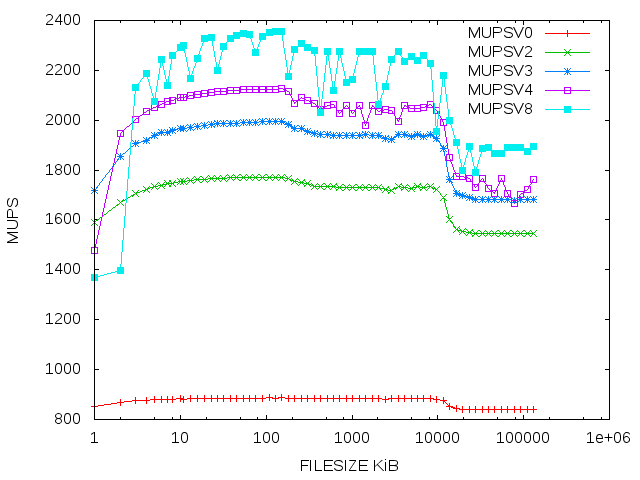
\includegraphics[scale=0.6]{pics/a3b.png}
	\caption{Plot of manual loop unrolling}
	\end{figure}
\end{center}

\subsection*{c)}
\begin{itemize}
	\item Geschwindigkeit steigt um $1.5$-fache pro Loop Unrolling ($8$-fache Loop-Unrolling \
		$\rightarrow$ $\approx4$-fache Geschwindigkeit)
	\item Sättigung tritt bereits bei Vektorgr\"osse von $10$ KiB auf. Danach aber kein
		Geschwindigkeitsverlust
	\item \textbf{Ursache:} Taktdauer von ADDSS?
\end{itemize}

\section*{Aufgabe 4}
\subsection*{b)}

\begin{center}
	\begin{figure}[h]
	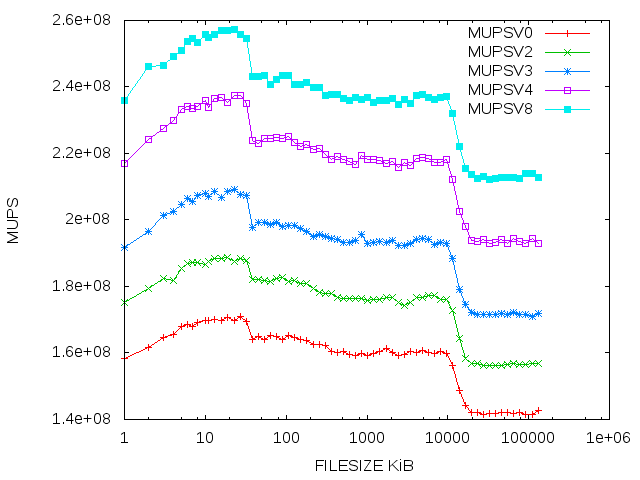
\includegraphics[scale=0.6]{pics/a4b.png}
	\caption{Plot of compiler based loop unrolling}
	\end{figure}
\end{center}

\subsection*{c)}
Cache Daten von Lima:\\
\begin{center}
	\begin{tabular}{| c || c |}
		\hline
		Cache-Typ             & Gr\"osse \\
		\hline
		\hline
		L1d cache             &    32K\\
		\hline
		L1i cache             &    32K\\
		\hline
		L2 cache              &    256K\\
		\hline
		L3 cache              &    12288K\\
		\hline
	\end{tabular}
\end{center}

\begin{itemize}
	\item Geschwindigkeit steigt um $0.2$-fache pro Loop Unrolling ($8$-fache Loop-Unrolling \
		$\rightarrow$ $\approx 1.2$-fache Geschwindigkeit)
	\item Maximale Geschwindkeit tritt bei Vektorgr\"osse von $\approx 50$ KiB auf.
		\begin{enumerate}
			\item Geschwindigkeitsverlust ab $50$ KiB\\ \textbf{Ursache:} Cache L1D voll
			\item Geschwindigkeitsverlust ab $10.000$ KiB\\ \textbf{Ursache:} Cache L3 voll
		\end{enumerate}
\end{itemize}

\end{document}
